\documentclass{beamer}

\mode<presentation>
{
  \usetheme{default}      % or try Darmstadt, Madrid, Warsaw, ...
  \usecolortheme{default} % or try albatross, beaver, crane, ...
  \usefonttheme{default}  % or try serif, structurebold, ...
  \setbeamertemplate{navigation symbols}{} % To remove the navigation symbols from the bottom of all slides uncomment this line
  \setbeamertemplate{footline}[page number] % To replace the footer line in all slides with a simple slide count uncomment this line
  \setbeamercolor{page number in head/foot}{fg=black}

} 
% For creating backup slides so that total # slides exclude backup slides, but the backup is still numbered
\newcommand{\backupbegin}{
   \newcounter{finalframe}
   \setcounter{finalframe}{\value{framenumber}}
}
\newcommand{\backupend}{
   \setcounter{framenumber}{\value{finalframe}}
}

% Packages
\usepackage[english]{babel}
\usepackage[utf8x]{inputenc}
\usepackage{graphicx} % Allows including images
\usepackage{booktabs} % Allows the use of \toprule, \midrule and \bottomrule in tables
\usepackage{tabto}
\usepackage[export]{adjustbox}
\usepackage{caption}
\usepackage{subcaption}
\usepackage{wrapfig}
\usepackage{multicol}
\usepackage{hyperref}
\usepackage{anyfontsize}
\usepackage{tcolorbox}
\usepackage{adjustbox}
\usepackage{tikzsymbols}
\usepackage{array}
\usepackage{amsmath}
\usepackage{hyperref}
\usepackage{listings}
\usepackage{xcolor}
\definecolor{olive}{rgb}{0.3, 0.4, .1}
\definecolor{fore}{RGB}{249,242,215}
\definecolor{back}{RGB}{51,51,51}
\definecolor{title}{RGB}{255,0,90}
\definecolor{dgreen}{rgb}{0.,0.6,0.}
\definecolor{gold}{rgb}{1.,0.84,0.}
\definecolor{JungleGreen}{cmyk}{0.99,0,0.52,0}
\definecolor{BlueGreen}{cmyk}{0.85,0,0.33,0}
\definecolor{RawSienna}{cmyk}{0,0.72,1,0.45}
\definecolor{Magenta}{cmyk}{0,1,0,0}
\usepackage{afterpage}

%---------------------------------------------------------------------------
%	TITLE PAGE
%---------------------------------------------------------------------------
\setbeamercolor{title}{fg=white}
\title[JET MASS  IN Z + JETS]{\textbf{UNFOLDING THE JET MASS  IN Z + JETS EVENTS }} % The short title appears at the bottom of every slide, the full title is only on the title page
\setbeamercolor{author}{fg=white}
\author{Christine McLean, Ashley Parker and Salvatore Rappoccio} % Your name
\setbeamercolor{institute}{fg=white}
\institute[University at Buffalo] % Your institution as it will appear on the bottom of every slide.
{
\textcolor{white}{\textit{ash.marie.parker@gmail.com}} % Your email address
}
\setbeamercolor{date}{fg=white}
\date{\today} % Date, can be changed to a custom date

% To left align title page contents
\makeatletter
\setbeamertemplate{title page}[default][left,colsep=-4bp,rounded=true,shadow=\beamer@themerounded@shadow]
\makeatother

\begin{document}

{
%%%%%%%%% Uncomment the below line to use UB-CMS template
\usebackgroundtemplate{
\includegraphics[width = 13.3cm, height = 9.6cm]{background/UB_background_title.pdf}}
%%%%%%%%% Uncomment the below line to use UB template
% \usebackgroundtemplate{
\includegraphics[width = 13.3cm, height = 9.6cm]{background/UBTemplate_titlepage.pdf}}

\begin{frame}[plain]
    \titlepage
\end{frame}
  }

%---------------------------------------------------------------------------
%	PRESENTATION SLIDES
%---------------------------------------------------------------------------
% setting background
%%%%%%%%% Uncomment the two lines below to use UB-CMS template
\usebackgroundtemplate{
\includegraphics[width = 12.8cm, height = 9.9cm]{background/background.pdf}}
\setbeamertemplate{frametitle}[default][center]% making all frame titles centered

%%%%%%%%% Uncomment the three lines below to use UB template
% \usebackgroundtemplate{
\includegraphics[width = 12.8cm, height = 9.9cm]{background/UBTemplate_background.pdf}}
% \setbeamertemplate{frametitle}[default][left]% making all frame titles centered
% \setbeamercolor{frametitle}{fg=white}
%----------------------------------------------------------------------------------------
\begin{frame}{\textbf{CMS AN-18-240}}
\vspace{3.5mm}
\begin{itemize}
\item A Measurement of normalized double differential jet production cross section in Z + Jet events :
\item[] $$ \frac{1}{ \frac{d\sigma}{dp_{T}} }   \frac{d^2\sigma}{dp_{T} dm}  (\frac{1}{GeV})  $$
\item We use TUnfoldDensity to perform 2D unfolding:
\item[] $$ ( p_{T} , [ m_u || m_g ] ) $$
\item We compare the ungroomed and groomed jet masses (9 combinations of the soft-drop parameters)
\item Today we show a preview of our preliminary results for 2017 data
\item Plan to publish this fall with 2016/2017/2018 or some subset of that data
\end{itemize}
\end{frame}
%----------------------------------------------------------------------------------------
\begin{frame}{\textbf{Motivation}}
\vspace{.9mm}
\centering
Jet Mass : A simple observable for testing QCD
\begin{figure}
\centering
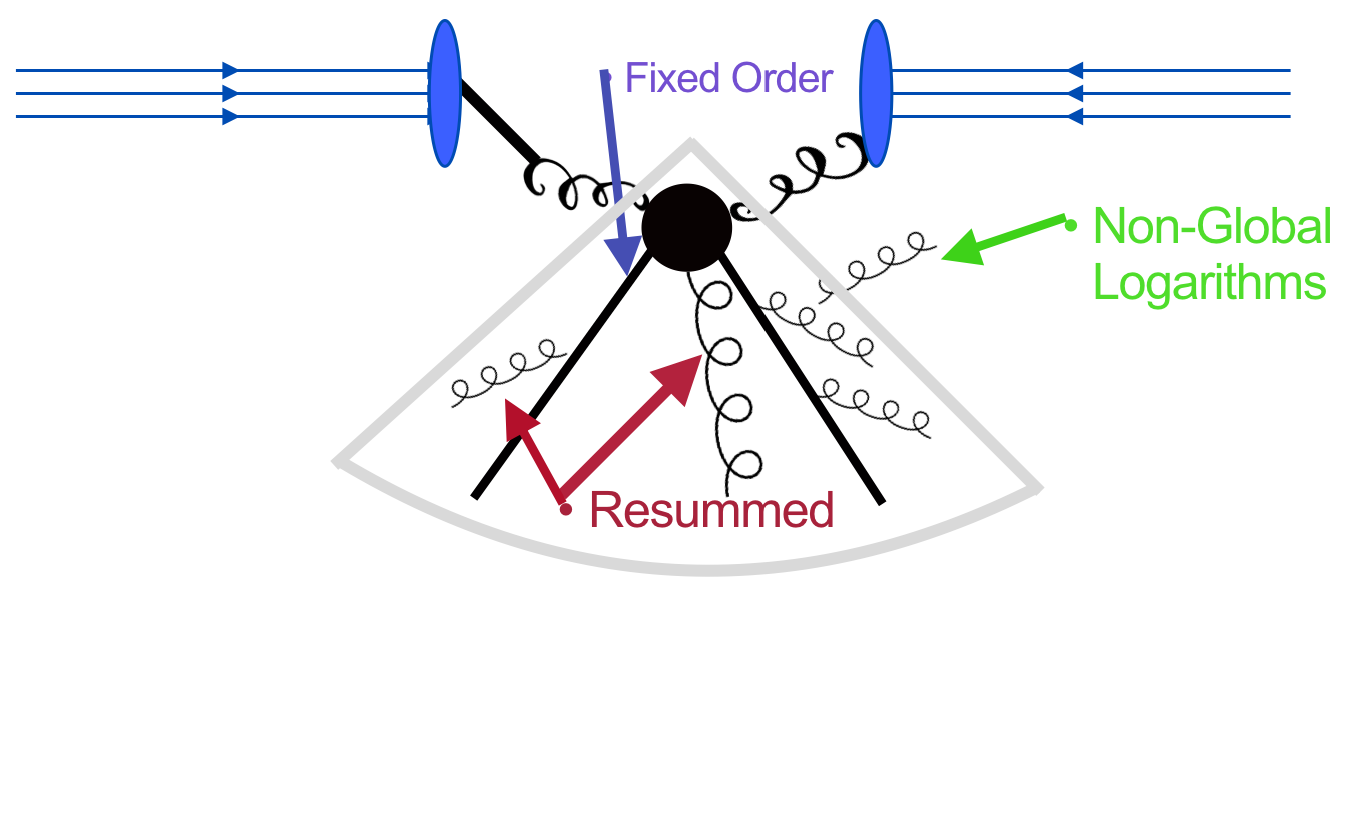
\includegraphics[scale=.27]{jet.png}
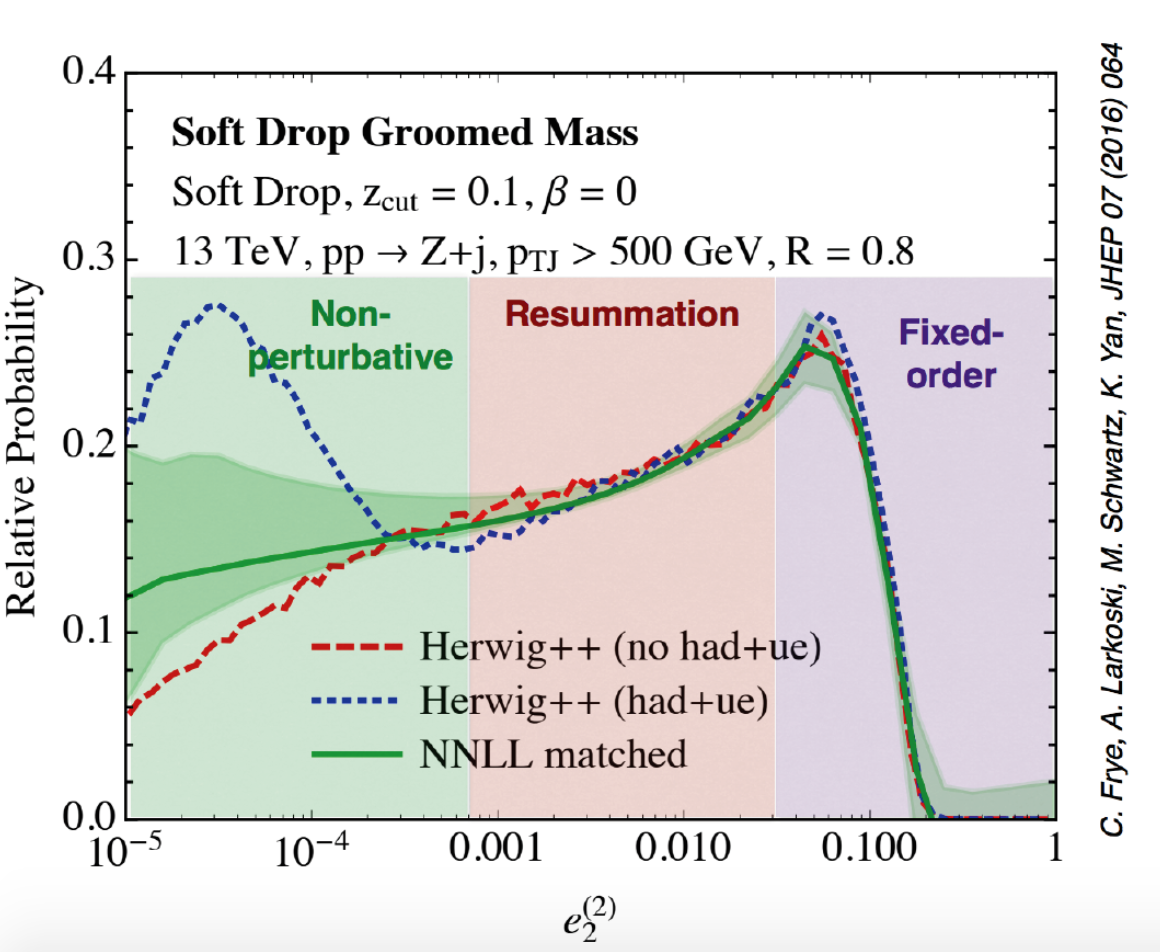
\includegraphics[scale=.25]{jetcalc.png}
\end{figure}
\begin{itemize}

\item Understand evolution of the “jet” function in perturbative QCD
\item Improve modeling of jets in Monte Carlo generators

\end{itemize}


\end{frame}




%----------------------------------------------------------------------------------------


%----------------------------------------------------------------------------------------
\begin{frame}{\textbf{Event Selection}}
\vspace{.9mm}
\centering
\begin{figure}
\centering
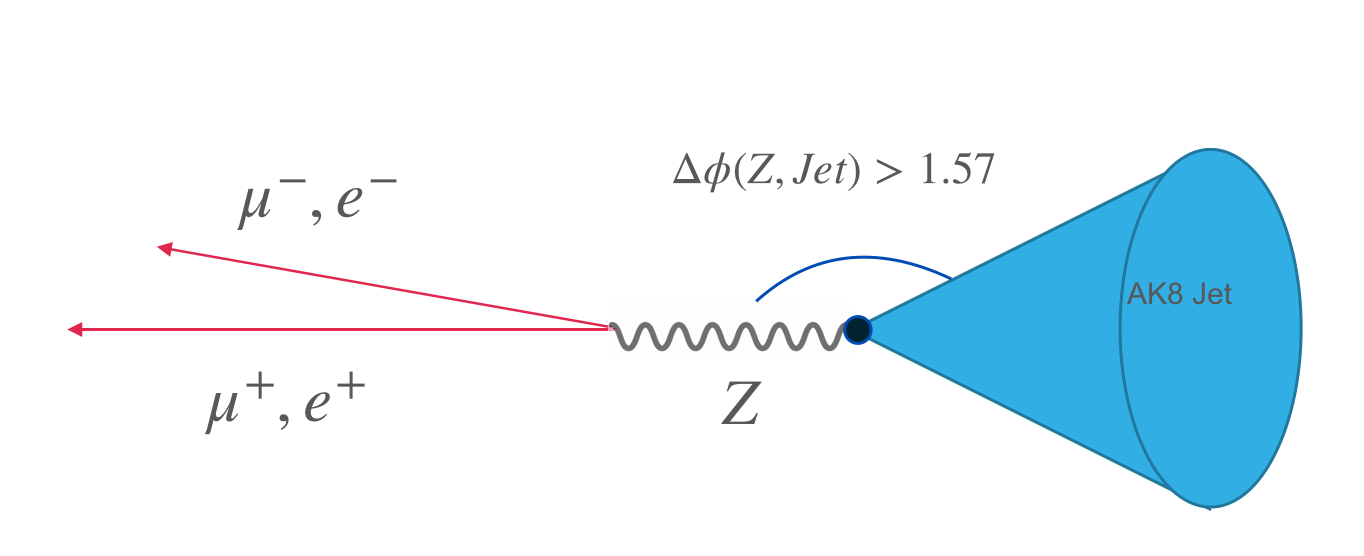
\includegraphics[scale=.35]{zjetevent.png}
\end{figure}



 \begin{block}{Summary}
\begin{itemize}
  \item At least 1 Anti-Kt $R = 0.8$ Jet, $P_T > 200 GeV $,  $|\eta| < 2.5 $, $dR(Jet, Lepton) > 0.8 $  
  \item 2 opposite sign, same flavor leptons, $|\eta| < 2.4 $
  \item Sum of the 2 leptons gives the Z candidate, $P_T > 90 GeV$,  $d\phi(Z, Jet) > 1.57$  

\end{itemize}

\end{block}







\end{frame}




%----------------------------------------------------------------------------------------


%----------------------------------------------------------------------------------------
\begin{frame}{\textbf{Event Selection}}

\begin{block}{Muons}
\begin{itemize}
  \item ISO     : PF relative Isolation 0.4 $< 0.25$ 
  \item ID      : Medium cut based ID 
  \item Trigger : IsoMu27 ($P_T > 29 GeV$)
\end{itemize}

\end{block}

\begin{block}{Electrons}
\begin{itemize}
  \item ISO     : None
  \item ID      : Medium cut based ID 
  \item Trigger : $Ele35_WPTight_Gsf OR Photon200$  ($P_T > 37 GeV$)
\end{itemize}

\end{block}



\end{frame}




%----------------------------------------------------------------------------------------



%----------------------------------------------------------------------------------------





\section{Unfolding}
%----------------------------------------------------------------------------------------
\begin{frame}{\textbf{Response Matrix}}
\vspace{.5mm}
%N

\begin{itemize}
  \item Normalized by Reconstructed (Y axis) $P_T$ bin
  \item Mass binning on X axis (Coarse/Output) :
  \item $[0.0, 10.0, 20.0, 40.0, 60.0, 80.0, 100.0, 150.0, 200.0, 13000.0]$
\end{itemize}


\begin{figure}
\centering
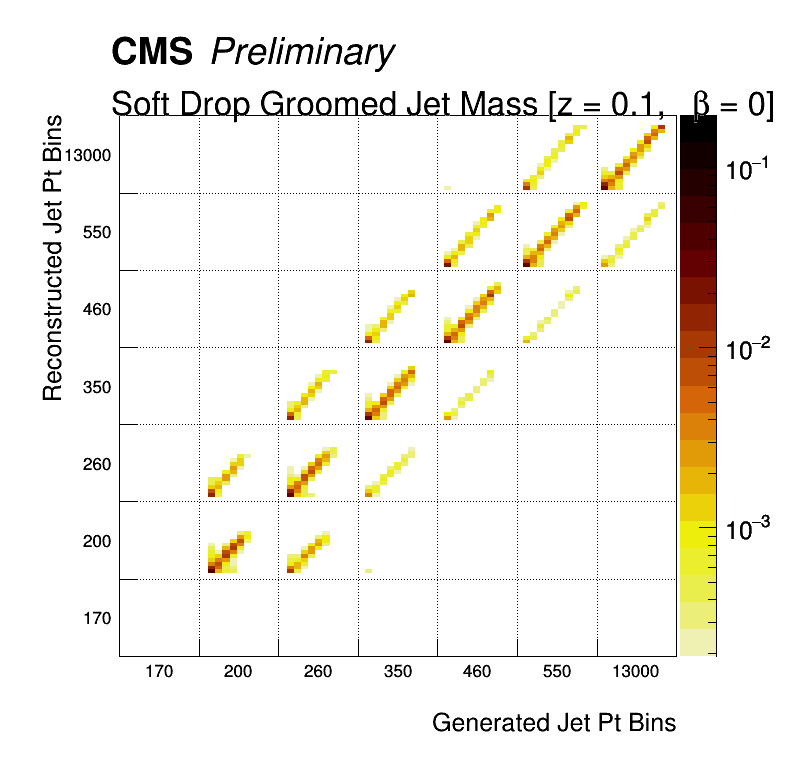
\includegraphics[scale=.25]{Oct31_unfoldPlots_sdB0/aResponseMatrix_NormalizedbyPtbin.png}
\end{figure}



\end{frame}
%----------------------------------------------------------------------------------------
%\section{Some \LaTeX{} Examples}

%------------------
\begin{frame}{\textbf{Purity and Stability of Binning Scheme}}



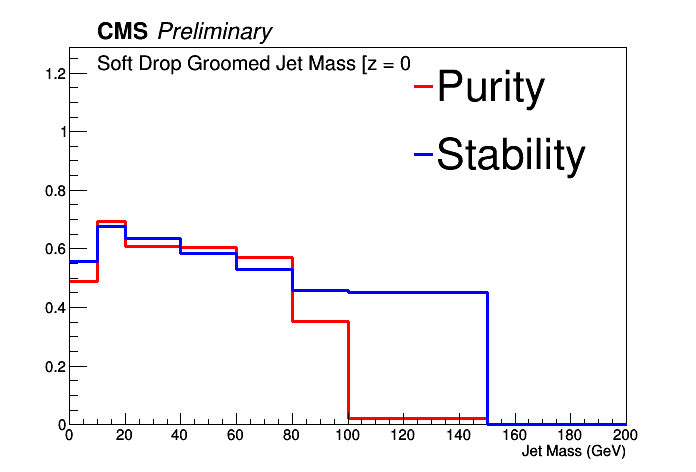
\includegraphics[width=0.5\textwidth]{Oct31_unfoldPlots_sdB0/PurityandStability_200_260.png}%
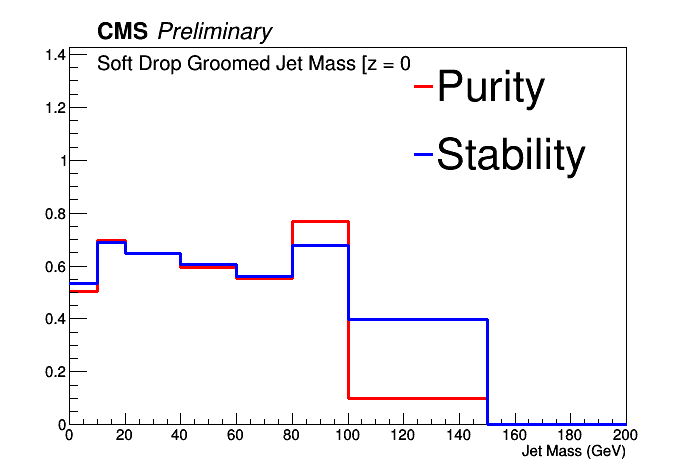
\includegraphics[width=0.5\textwidth]{Oct31_unfoldPlots_sdB0/PurityandStability_260_350.png}
\newline
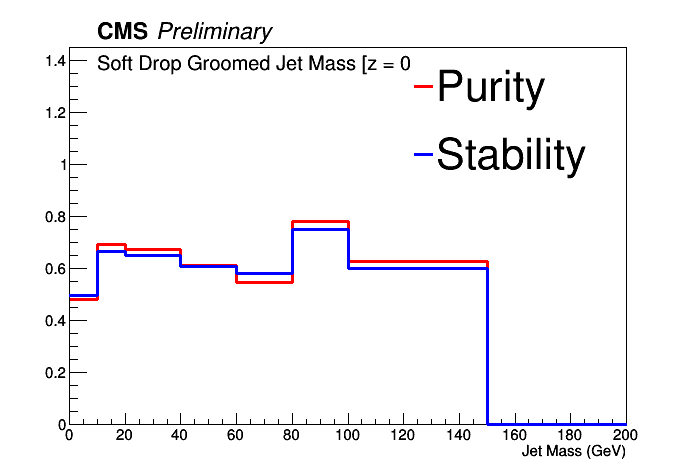
\includegraphics[width=0.3333\textwidth]{Oct31_unfoldPlots_sdB0/PurityandStability_350_460.png}%
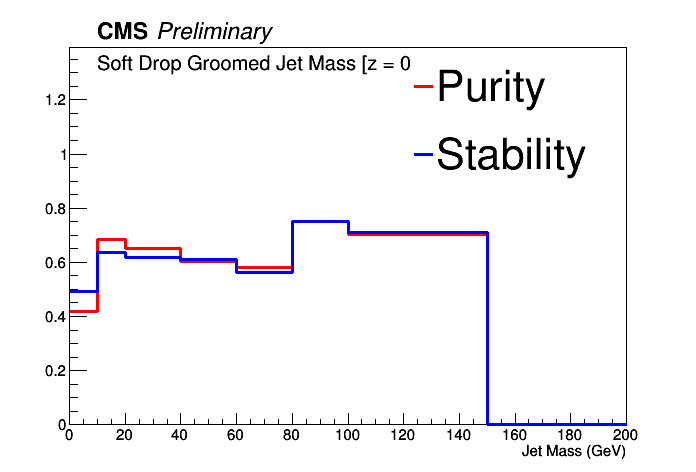
\includegraphics[width=0.3333\textwidth]{Oct31_unfoldPlots_sdB0/PurityandStability_460_550.png}
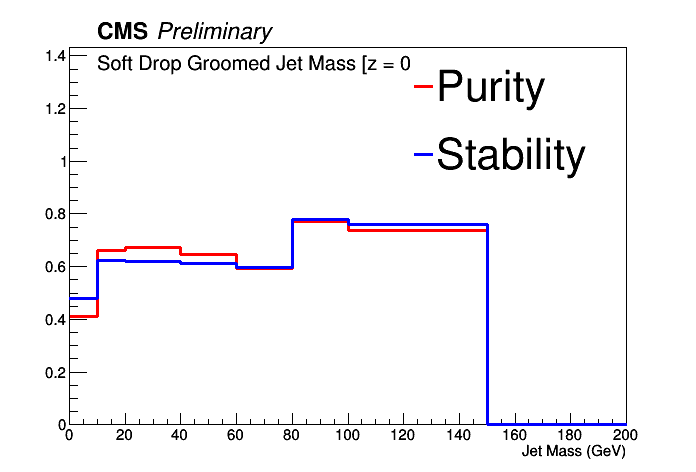
\includegraphics[width=0.3333\textwidth]{Oct31_unfoldPlots_sdB0/PurityandStability_550_13000.png}




\end{frame}
%----------------------------------------------------------------------------------------


\subsection{Input Distributions}

%----------------------------------------------------------------------------------------
\begin{frame}{\textbf{2017 Input MC}}



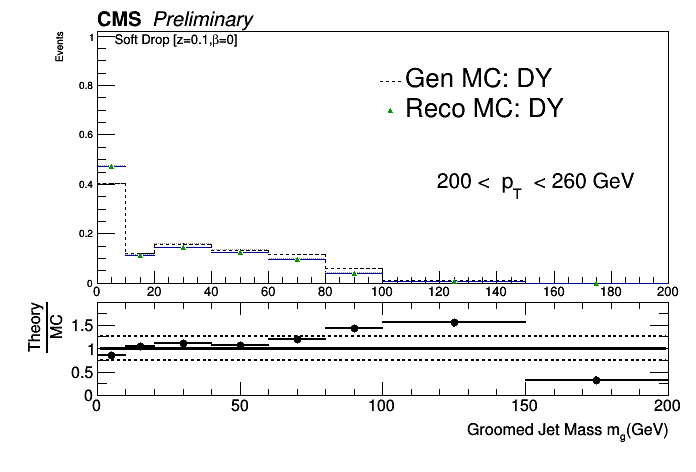
\includegraphics[width=0.5\textwidth]{Oct31_unfoldPlots_sdB0/InputlocalrecobinnedMC_mass_Ptbin200to260_Detbinning_Groomingis_sdB0.png}%
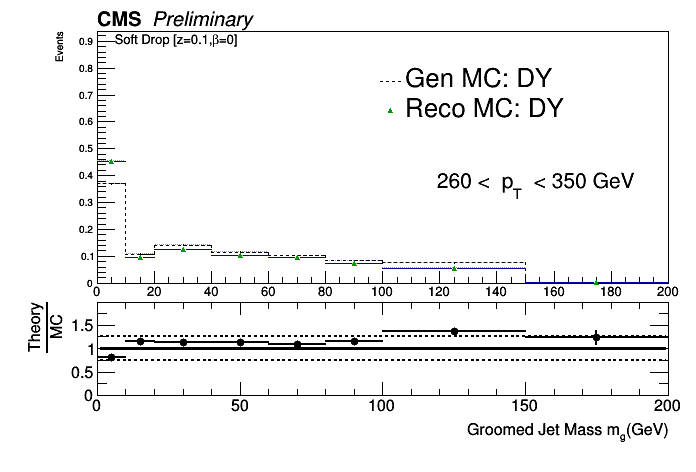
\includegraphics[width=0.5\textwidth]{Oct31_unfoldPlots_sdB0/InputlocalrecobinnedMC_mass_Ptbin260to350_Detbinning_Groomingis_sdB0.png}
\newline
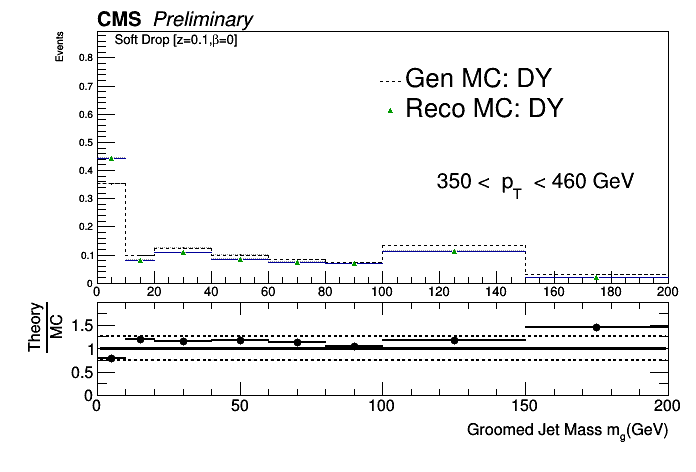
\includegraphics[width=0.3333\textwidth]{Oct31_unfoldPlots_sdB0/InputlocalrecobinnedMC_mass_Ptbin350to460_Detbinning_Groomingis_sdB0.png}%
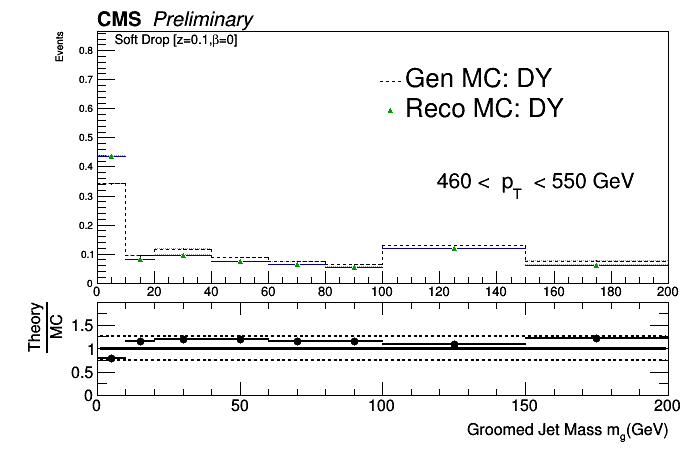
\includegraphics[width=0.3333\textwidth]{Oct31_unfoldPlots_sdB0/InputlocalrecobinnedMC_mass_Ptbin460to550_Detbinning_Groomingis_sdB0.png}
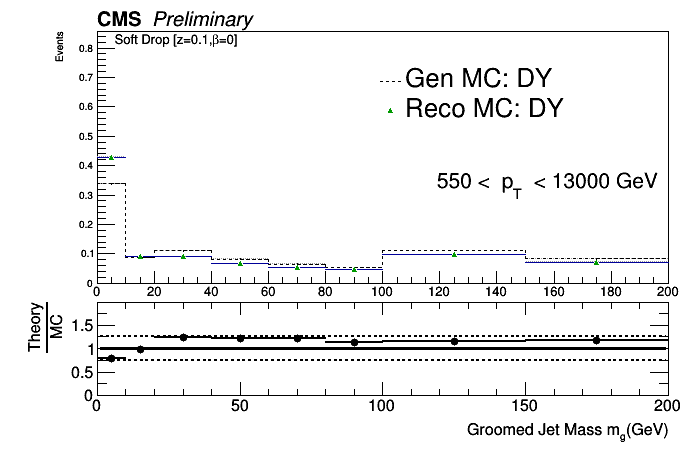
\includegraphics[width=0.3333\textwidth]{Oct31_unfoldPlots_sdB0/InputlocalrecobinnedMC_mass_Ptbin550to13000_Detbinning_Groomingis_sdB0.png}
%\begin{columns}[t]
%        \column{.5\textwidth}
%        \includegraphics[width=\columnwidth,height=1cm]%{Oct31_unfoldPlots_sdB0/InputlocalrecobinnedMC_mass_Ptbin200to260_Detbinning_Groomingis_sdB0.png}
        %\captionof{figure}{foo}
%        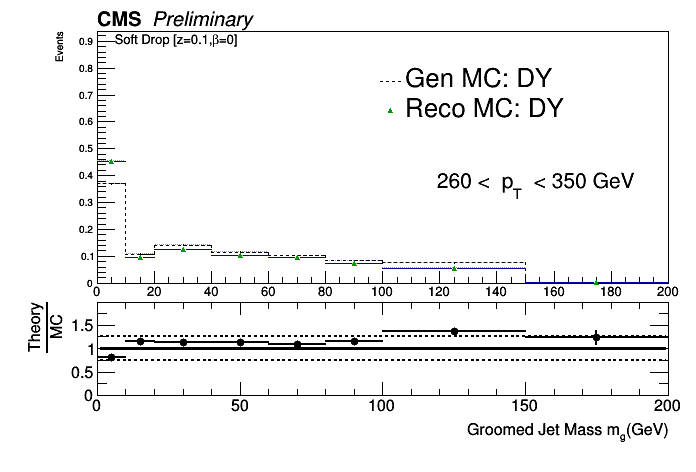
\includegraphics[width=\columnwidth,height=1cm]{Oct31_unfoldPlots_sdB0/InputlocalrecobinnedMC_mass_Ptbin260to350_Detbinning_Groomingis_sdB0.png}        
%        %\captionof{figure}{bar}
%        \column{.5\textwidth}
%        \includegraphics[width=\columnwidth,height=1cm]%{Oct31_unfoldPlots_sdB0/InputlocalrecobinnedMC_mass_Ptbin350to460_Detbinning_Groomingis_sdB0.png}        
%        %\captionof{figure}{foo}
%        \includegraphics[width=\columnwidth,height=1cm]%{Oct31_unfoldPlots_sdB0/InputlocalrecobinnedMC_mass_Ptbin460to550_Detbinning_Groomingis_sdB0.png}        
%$        %\captionof{figure}{bar}%
%
        %\captionof{figure}{foo}
%\end{columns}


\end{frame}
%----------------------------------------------------------------------------------------

%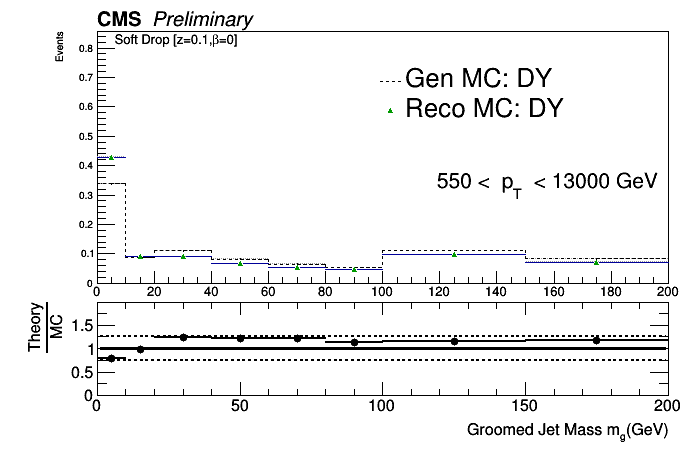
\includegraphics[width=\columnwidth,height=3cm]{Oct31_unfoldPlots_sdB0/InputlocalrecobinnedMC_mass_Ptbin550to13000_Detbinning_Groomingis_sdB0.png} 
%\begin{figure}
%5\centering
%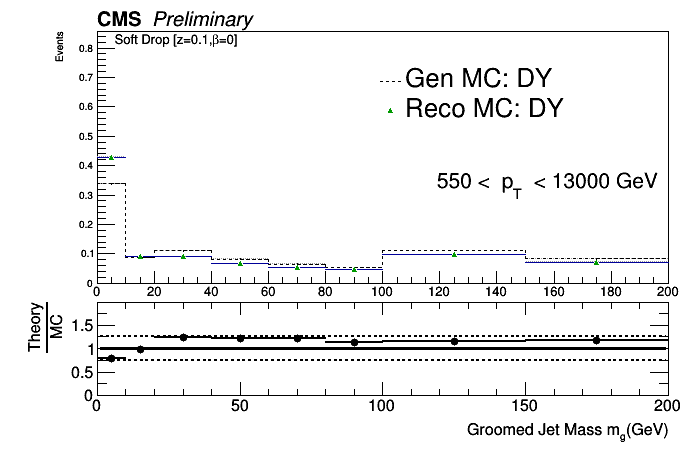
\includegraphics[scale=.27]{Oct31_unfoldPlots_sdB0/InputlocalrecobinnedMC_mass_Ptbin550to13000_Detbinning_Groomingis_sdB0.png}
%\end{figure}



\subsection{Closure}

%------------------
\begin{frame}{\textbf{2017 MC Closure Test}}

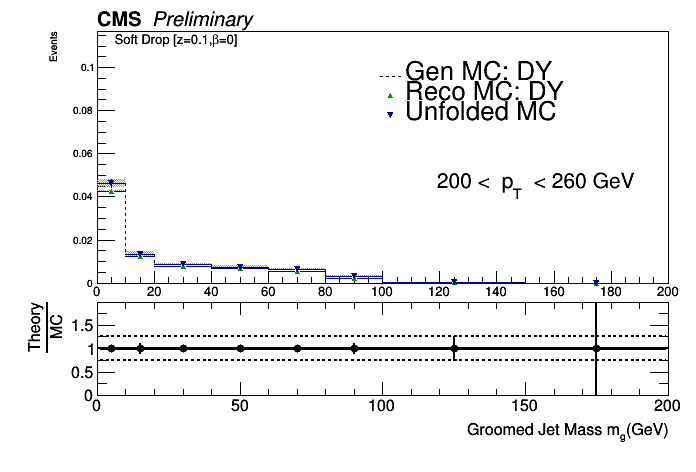
\includegraphics[width=0.5\textwidth]{Oct31_unfoldPlots_sdB0/Output_NoReg_MC_ptbin1MC_mass_Ptbin200to260_Detbinning_Groomingis_sdB0.png}%
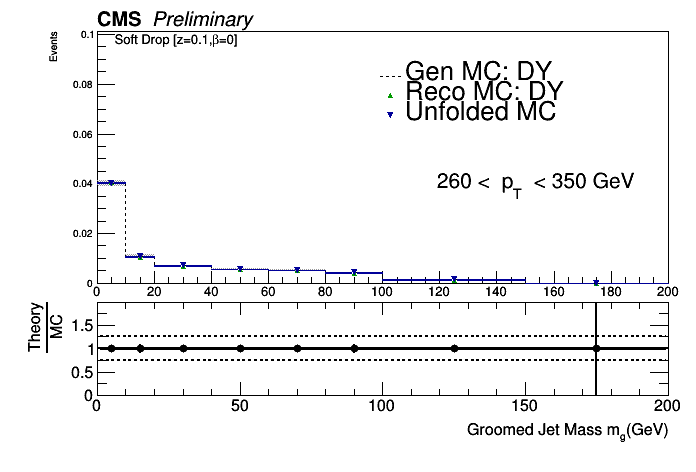
\includegraphics[width=0.5\textwidth]{Oct31_unfoldPlots_sdB0/Output_NoReg_MC_ptbin2MC_mass_Ptbin260to350_Detbinning_Groomingis_sdB0.png}
\newline
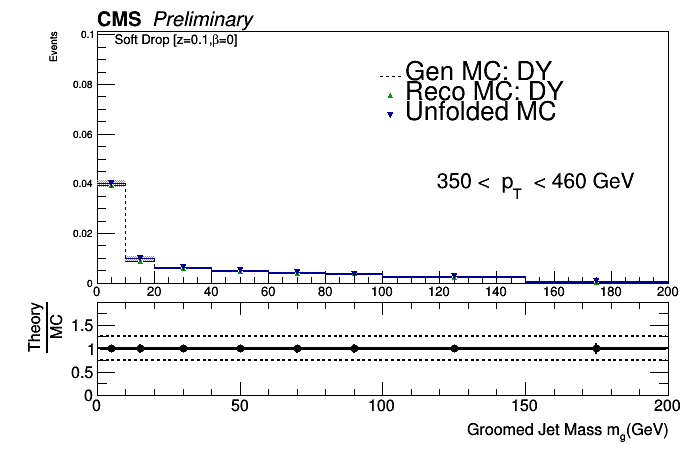
\includegraphics[width=0.3333\textwidth]{Oct31_unfoldPlots_sdB0/Output_NoReg_MC_ptbin3MC_mass_Ptbin350to460_Detbinning_Groomingis_sdB0.png}%
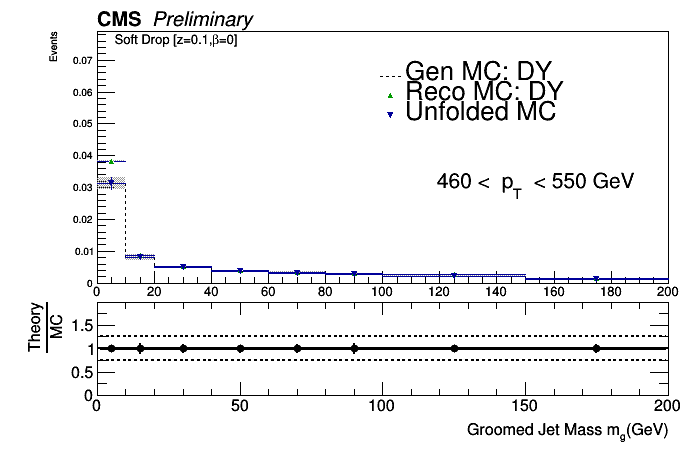
\includegraphics[width=0.3333\textwidth]{Oct31_unfoldPlots_sdB0/Output_NoReg_MC_ptbin4MC_mass_Ptbin460to550_Detbinning_Groomingis_sdB0.png}
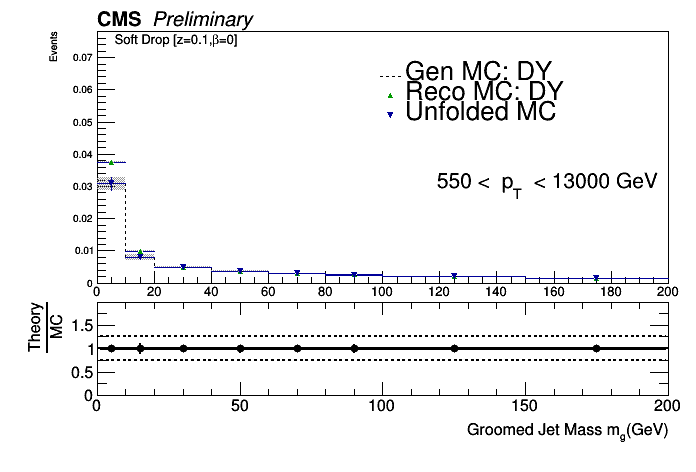
\includegraphics[width=0.3333\textwidth]{Oct31_unfoldPlots_sdB0/Output_NoReg_MC_ptbin5MC_mass_Ptbin550to13000_Detbinning_Groomingis_sdB0.png}





\end{frame}
%----------------------------------------------------------------------------------------

%------------------
\begin{frame}{\textbf{2017 Data and MC Luminosities}}

 \begin{table}
\centering
\begin{tabular}{l|r}
Drell-Yan HT bin (GeV) & Fraction of Data Luminosity (41.3 $fb^(-1)$)\\\hline
100-200 & 2.1 \\
200-400 & 5.6 \\
400-600 & 33.9 \\
600-800 & 111.0 \\
800-1200 & 87.8 \\
1200-2500 & 817.8 \\
2500-Inf & 2685.28 \\


\end{tabular}
\caption{\label{tab:datamclumi} The ratio of effective luminosity in data as compared to MC where $ L = \sigma * N_{events}$.}
\end{table}
 
 



\end{frame}
%----------------------------------------------------------------------------------------
%------------------
\begin{frame}{\textbf{Systematic Uncertanties}}
\begin{itemize}
  \item Used TUnfoldSys to propogate uncertanties 
  \item Input response matrices filled with observables shifted up and down 1 $\sigma$ from nominal 
  \item  Physics Model, JEC, JER, JMR, JMS, PU, PDF
  \item Compare to Dijet uncertanties from SMP-16-10 on next slides
\end{itemize}

\begin{block}{Ongoing Work}
\begin{itemize}
  \item Statistical uncertainy estimation using jacknife resampling
%  \item Updating to Fall17\_17Nov2017\_V32 JECs 
%  \item Adding extension samples to Drell-Yan signal MC in increase statistics
\end{itemize}

\end{block}


\end{frame}
%----------------------------------------------------------------------------------------

%------------------
\begin{frame}{\textbf{Systematic Uncertanties: Z+Jets and DiJets}}

\vspace{.5mm}
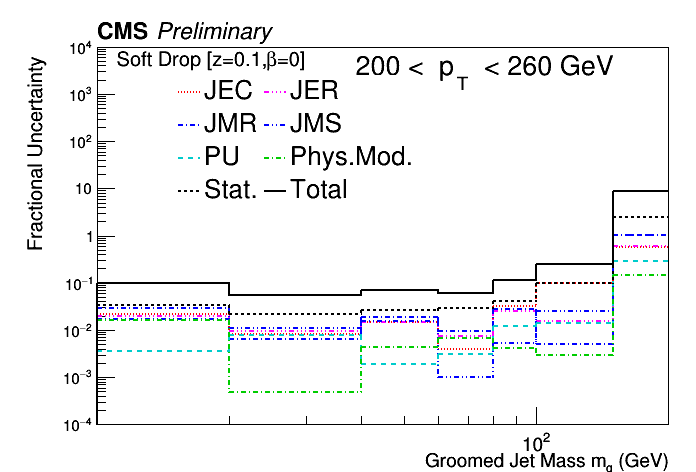
\includegraphics[width=0.5\textwidth]{Oct31_unfoldPlots_sdB0/AllSystematics_FractionofUnfoldedBinContent_ptbin2MC_mass_Ptbin200to260_Detbinning_Groomingis_sdB0.png}%
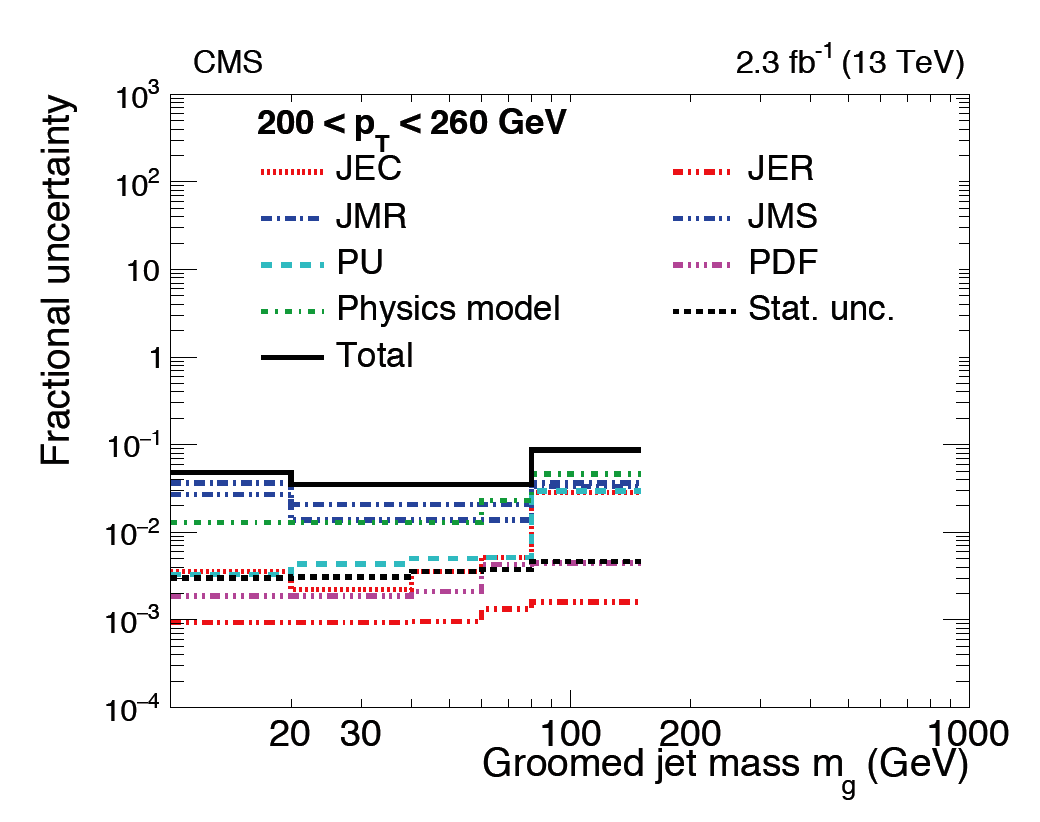
\includegraphics[width=0.4\textwidth]{dijet200.png}
\newline
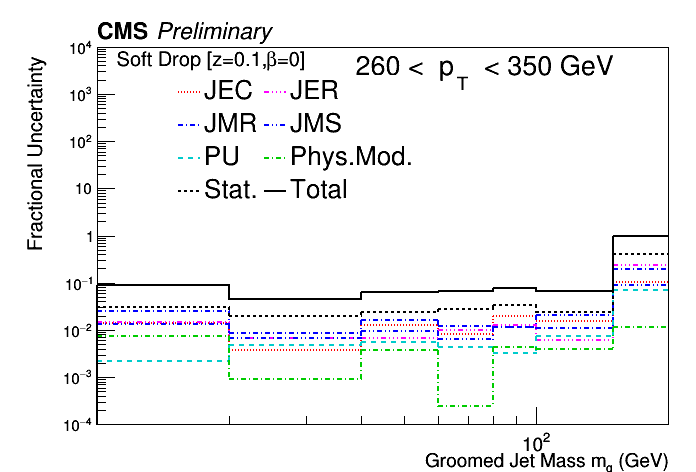
\includegraphics[width=0.5\textwidth]{Oct31_unfoldPlots_sdB0/AllSystematics_FractionofUnfoldedBinContent_ptbin3MC_mass_Ptbin260to350_Detbinning_Groomingis_sdB0.png}%
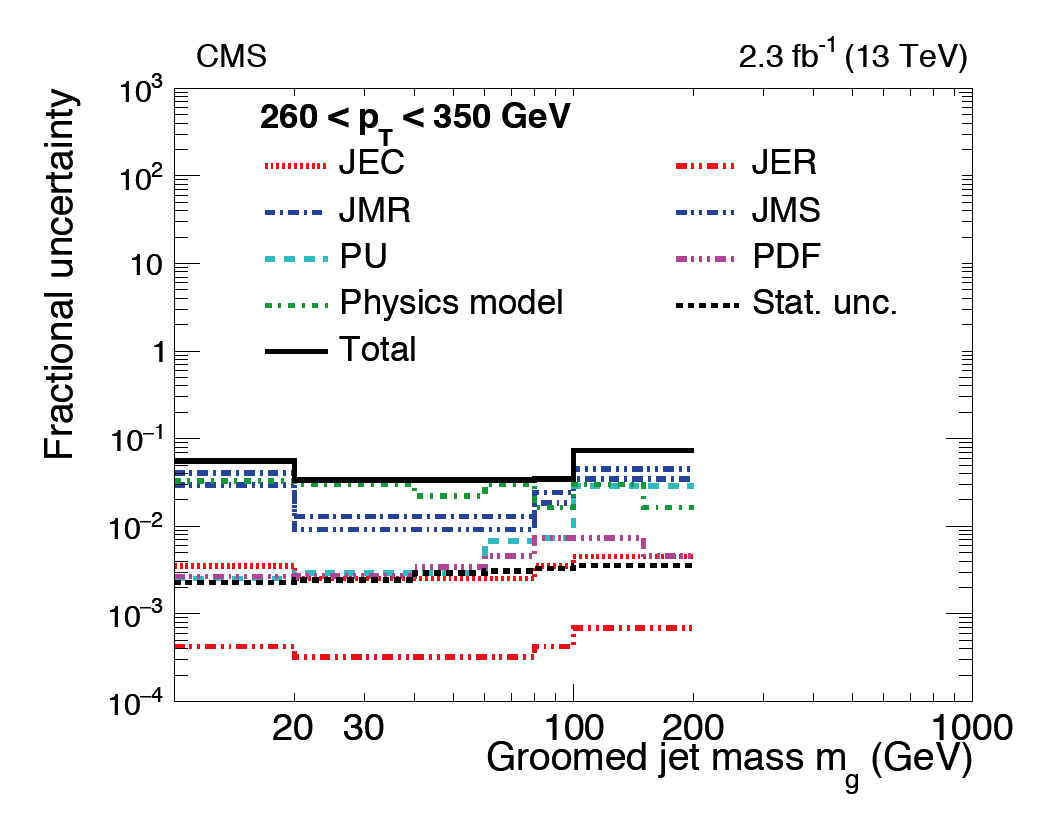
\includegraphics[width=0.4\textwidth]{dijet260.png}


\end{frame}
%----------------------------------------------------------------------------------------


%------------------
\begin{frame}{\textbf{Systematic Uncertanties: Z+Jets and DiJets}}


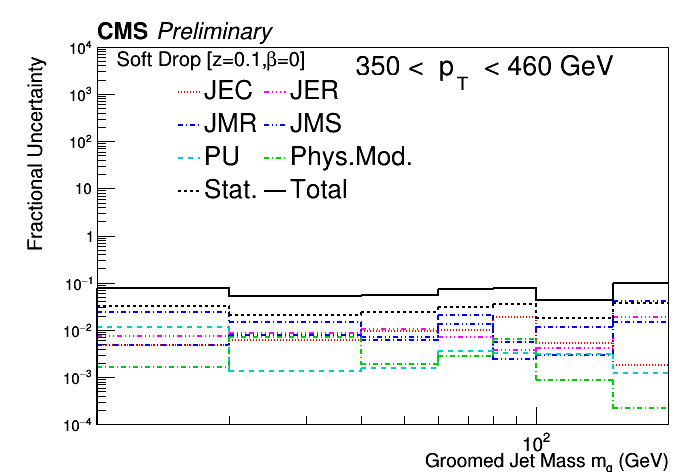
\includegraphics[width=0.5\textwidth]{Oct31_unfoldPlots_sdB0/AllSystematics_FractionofUnfoldedBinContent_ptbin4MC_mass_Ptbin350to460_Detbinning_Groomingis_sdB0.png}%
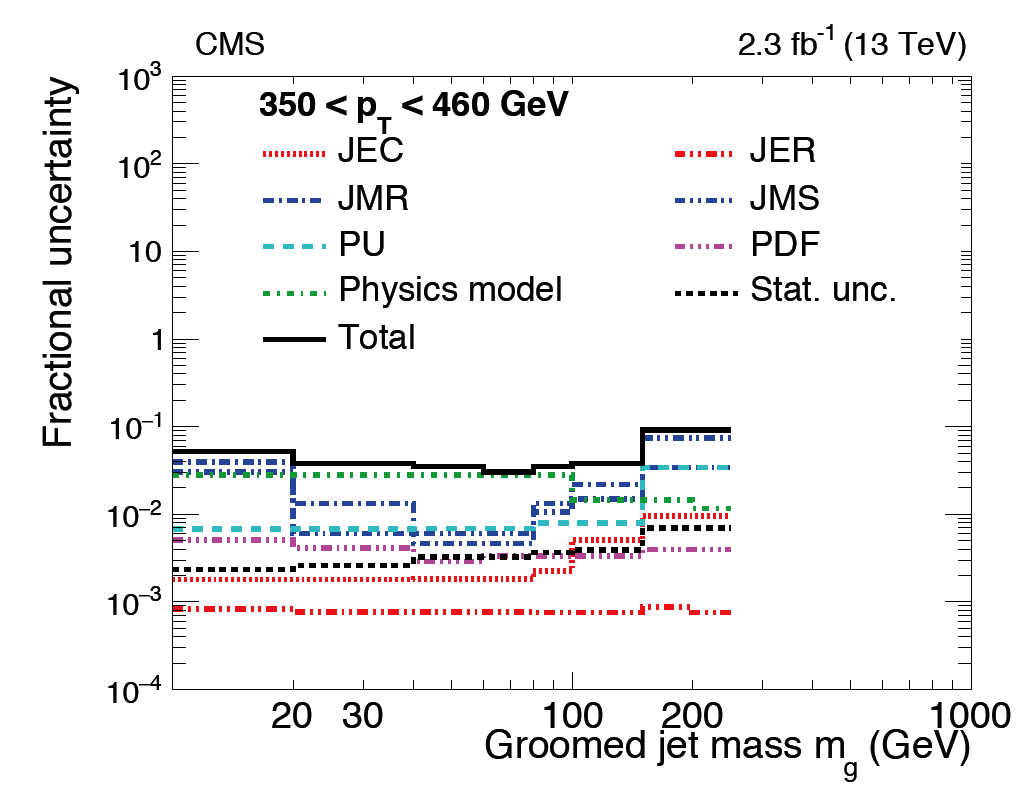
\includegraphics[width=0.4\textwidth]{dijet350.png}
\newline
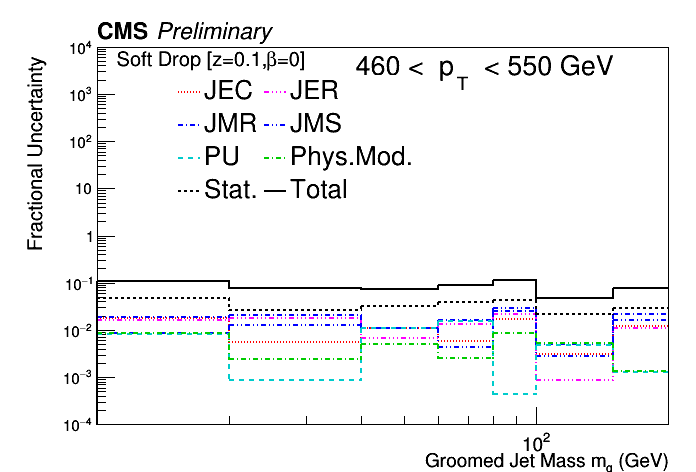
\includegraphics[width=0.5\textwidth]{Oct31_unfoldPlots_sdB0/AllSystematics_FractionofUnfoldedBinContent_ptbin5MC_mass_Ptbin460to550_Detbinning_Groomingis_sdB0.png}%
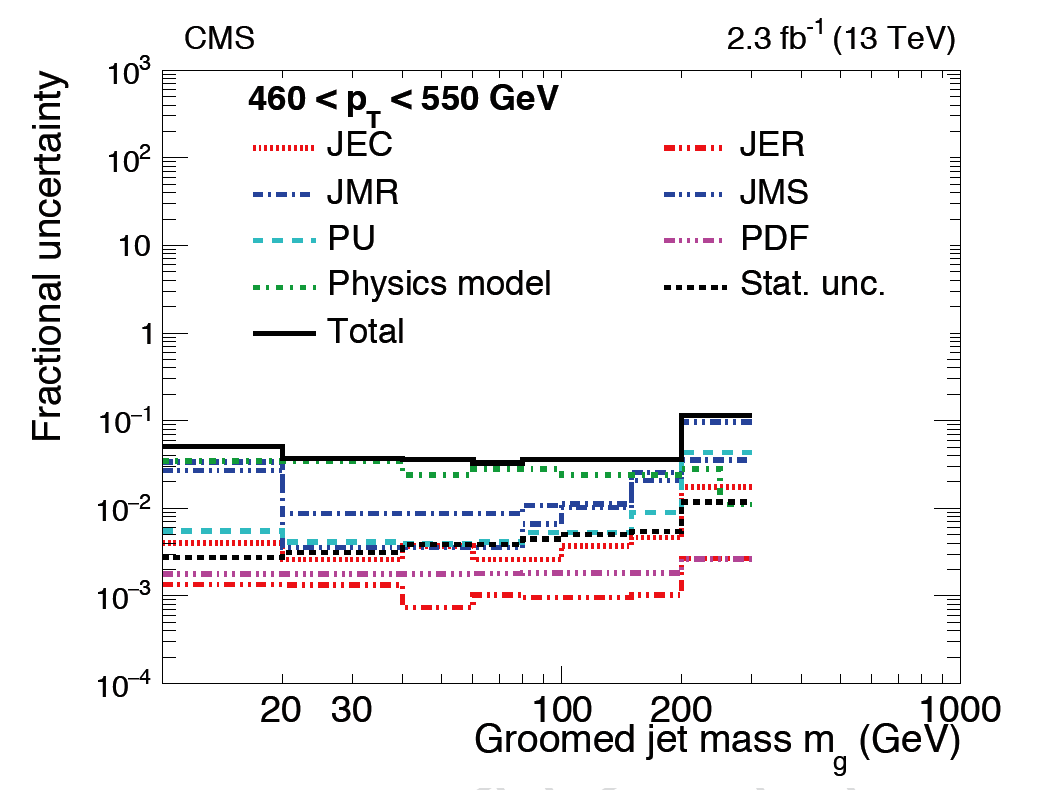
\includegraphics[width=0.4\textwidth]{dijet460.png}

%\includegraphics[width=0.5\textwidth]{fff}


\end{frame}
%----------------------------------------------------------------------------------------


%------------------
\begin{frame}{\textbf{Systematic Uncertanties: Z+Jets and DiJets}}


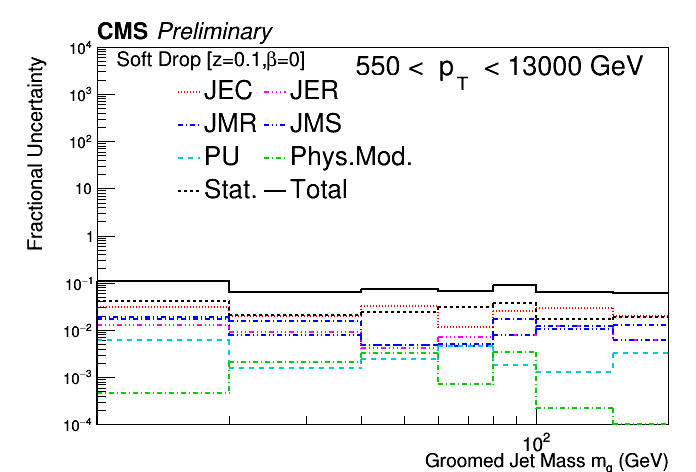
\includegraphics[width=0.55\textwidth]{Oct31_unfoldPlots_sdB0/AllSystematics_FractionofUnfoldedBinContent_ptbin6MC_mass_Ptbin550to13000_Detbinning_Groomingis_sdB0.png}%
\newline
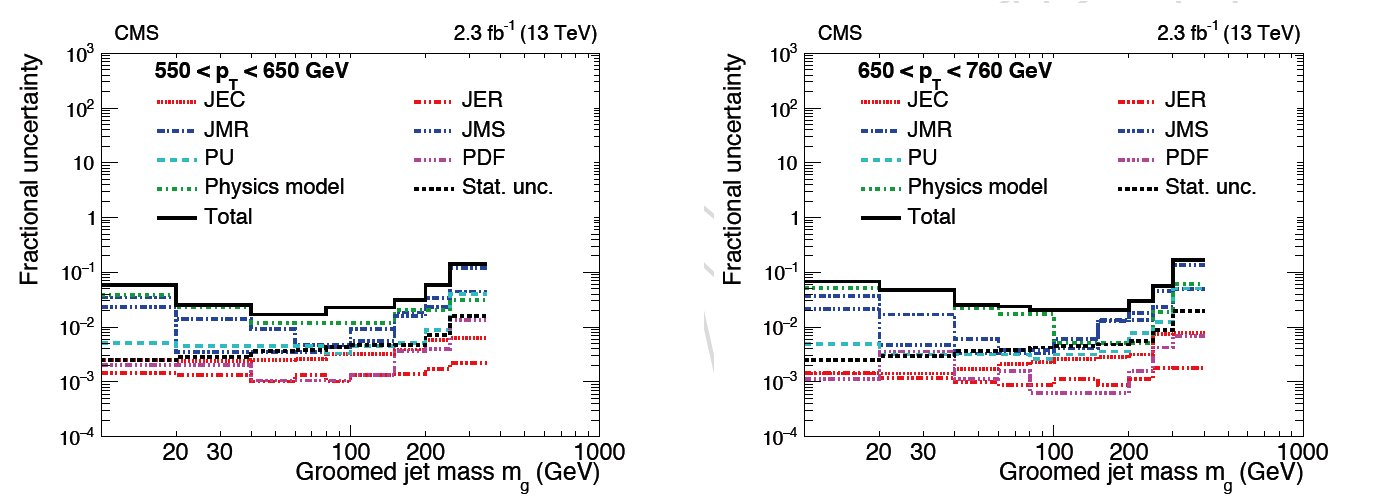
\includegraphics[width=1\textwidth]{dijet550andup.png}
\newline


\end{frame}
%----------------------------------------------------------------------------------------

\begin{frame}{\textbf{Summary : AN-18-240}}
\vspace{3.5mm}
\begin{itemize}
\item A Measurement of normalized double differential jet production cross section in Z + Jet events :
\item[] $$ \frac{1}{ \frac{d\sigma}{dp_{T}} }   \frac{d^2\sigma}{dp_{T} dm}  (\frac{1}{GeV})  $$

\item Method is complete and systematic uncertanites are understood
\item Plan to publish this fall with 2016/2017/2018 or some subset of that data




\end{itemize}
\end{frame}


%----------------------------------------------------------------------------------------

{\usebackgroundtemplate{}
\begin{frame}
\Huge{\centerline{The End}}
\end{frame}}
\appendix
\backupbegin

%----------------------------------------------------------------------------------------
% {\usebackgroundtemplate{}
% \begin{frame}
% \Huge{\centerline{Backup}}
% \end{frame}}
%----------------------------------------------------------------------------------------
\begin{frame}{\textbf{Extra Stuff}}
\vspace{3.5mm}
%Something I wanted to keep in backup because I thought it was cool.
\end{frame}
%----------------------------------------------------------------------------------------
\backupend

\end{document}
